\documentclass[11pt,a4paper]{article}

\usepackage[margin=1in]{geometry}
\usepackage{mathptmx}
\usepackage{amsmath}
\usepackage{amssymb}
\usepackage{amsthm}
\usepackage{braket}
\usepackage{tikz}
\usetikzlibrary{shapes.geometric}
\usepackage{quantikz}
\usepackage{enumitem}
\usepackage{hyperref}
\usepackage{xcolor}

\definecolor{circuitblue}{RGB}{40,80,160}

\hypersetup{
    colorlinks=true,
    linkcolor=circuitblue,
    urlcolor=circuitblue,
    citecolor=circuitblue
}

\theoremstyle{definition}
\newtheorem{definition}{Definition}[section]
\newtheorem{example}{Example}[section]
\newtheorem{theorem}{Theorem}[section]

\theoremstyle{remark}
\newtheorem*{intuition}{Intuition}
\newtheorem*{keypoint}{Key Point}

\pagestyle{plain}

\setlength{\parindent}{0pt}
\setlength{\parskip}{6pt}

\begin{document}

\begin{center}
    {\LARGE \textbf{Quantum Kernels in Practice}}\\[8pt]
    {\large QML}\\[12pt]
    \hrule
\end{center}

\vspace{12pt}
\tableofcontents
\newpage

%% ========================================================
\section{Overview}
%% ========================================================

last lecture we built up the theory of quantum kernels --- quantum feature maps, the kernel trick in hilbert space, and the connection between variational circuits and kernel methods. now its time to actually \emph{use} all that. this lecture is the practical follow-up: we go from theory to implementation.

we r going to walk through the full pipeline of implementing quantum kernels in qiskit, using them with scikit-learn SVMs, and benchmarking them against classical kernels on real (well, toy) datasets. this is the lecture where u actually learn how to build smtg that runs.

the main topics:
\begin{itemize}[leftmargin=*]
    \item how to implement quantum kernels step by step in qiskit
    \item the \texttt{FidelityQuantumKernel} class and wt it does internally
    \item choosing feature maps --- which ones work, which ones dont, and why
    \item computing the kernel matrix in practice --- shots, noise, statistical errors
    \item plugging quantum kernels into sklearn's SVM (QSVC, QSVR)
    \item kernel alignment --- the metric that tells u if ur kernel is any good
    \item practical considerations: qubits, depth, noise
    \item benchmarking on iris, moons, and circles datasets
\end{itemize}

tbh this is where quantum kernels either impress u or disappoint u. spoiler: on small toy datasets, they work fine but dont beat classical methods. the real question is whether they can do smtg classical kernels cant on structured problems.

%% ========================================================
\section{The Full Quantum Kernel Pipeline}
%% ========================================================

before we dive into code details, lets see the big picture. the full workflow from raw data to prediction looks like this:

\begin{center}
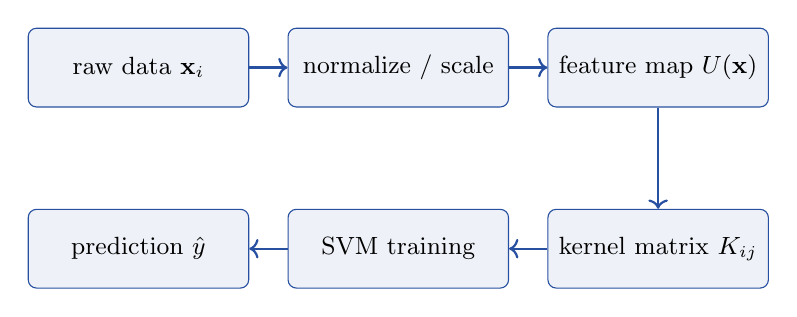
\begin{tikzpicture}[
    node distance=1.8cm,
    block/.style={rectangle, draw=circuitblue, fill=circuitblue!8,
        minimum width=2.8cm, minimum height=1cm, rounded corners=3pt,
        font=\small},
    arrow/.style={->, thick, circuitblue}
]
    \node[block] (data) {raw data $\mathbf{x}_i$};
    \node[block, right of=data, xshift=1.5cm] (norm) {normalize / scale};
    \node[block, right of=norm, xshift=1.5cm] (fmap) {feature map $U(\mathbf{x})$};
    \node[block, below of=fmap, yshift=-0.5cm] (kernel) {kernel matrix $K_{ij}$};
    \node[block, left of=kernel, xshift=-1.5cm] (svm) {SVM training};
    \node[block, left of=svm, xshift=-1.5cm] (pred) {prediction $\hat{y}$};

    \draw[arrow] (data) -- (norm);
    \draw[arrow] (norm) -- (fmap);
    \draw[arrow] (fmap) -- (kernel);
    \draw[arrow] (kernel) -- (svm);
    \draw[arrow] (svm) -- (pred);
\end{tikzpicture}
\end{center}

each step matters. if u mess up the normalization, ur feature map wont work well. if u choose a bad feature map, ur kernel matrix will be garbage. if u dont use enough shots, ur kernel entries will be noisy. lets go through each piece.

\subsection{Step 1: Data Preprocessing}

quantum feature maps typically encode data into rotation angles. this means ur data needs to be in a range thats compatible with rotation gates --- usually $[0, 2\pi]$ or $[-\pi, \pi]$.

\begin{keypoint}
always normalize ur data before feeding it to a quantum kernel. the standard approach is min-max scaling to $[0, \pi]$ or standardization followed by a sigmoid-like compression. if u skip this, ur rotation gates will either saturate (everything maps to roughly the same state) or underuse the available range.
\end{keypoint}

the preprocessing pipeline:
\begin{enumerate}[leftmargin=*]
    \item start with raw features $\mathbf{x} \in \mathbb{R}^d$
    \item apply standard scaling: $\mathbf{x} \to \frac{\mathbf{x} - \mu}{\sigma}$
    \item rescale to $[0, \pi]$: $\mathbf{x} \to \pi \cdot \frac{\mathbf{x} - \mathbf{x}_{\min}}{\mathbf{x}_{\max} - \mathbf{x}_{\min}}$
    \item if $d > n_{\text{qubits}}$, apply PCA to reduce dimensionality first
\end{enumerate}

\subsection{Step 2: Define the Feature Map Circuit}

the feature map $U(\mathbf{x})$ is a parameterized quantum circuit that encodes classical data into quantum states. in qiskit, u create this using the circuit library.

the standard approach: create a \texttt{ZZFeatureMap} or \texttt{ZFeatureMap} from \texttt{qiskit.circuit.library}. u specify the number of qubits, the number of repetitions (called ``reps''), and the entanglement pattern.

\begin{definition}[Quantum Feature Map Circuit]
a quantum feature map is a unitary $U(\mathbf{x})$ applied to $\ket{0}^{\otimes n}$ to produce the quantum state
\[
\ket{\phi(\mathbf{x})} = U(\mathbf{x})\ket{0}^{\otimes n}
\]
the corresponding quantum kernel is
\[
\kappa(\mathbf{x}, \mathbf{x}') = |\braket{\phi(\mathbf{x})|\phi(\mathbf{x}')}|^2 = |\bra{0}^{\otimes n} U^\dagger(\mathbf{x}) U(\mathbf{x}') \ket{0}^{\otimes n}|^2
\]
\end{definition}

here is the circuit that computes this kernel entry:

\begin{center}
\begin{quantikz}
    \lstick{$\ket{0}$} & \gate{U(\mathbf{x}')} & \gate{U^\dagger(\mathbf{x})} & \meter{} \\
    \lstick{$\ket{0}$} & \gate{U(\mathbf{x}')} & \gate{U^\dagger(\mathbf{x})} & \meter{} \\
    \lstick{$\ket{0}$} & \gate{U(\mathbf{x}')} & \gate{U^\dagger(\mathbf{x})} & \meter{}
\end{quantikz}
\end{center}

the kernel value is the probability of measuring $\ket{0}^{\otimes n}$ at the output. if the two data points r similar, the states r similar, the inverse maps back close to $\ket{0}^{\otimes n}$, and u get a high probability. if theyre different, u get a low probability.

%% ========================================================
\section{The FidelityQuantumKernel Class}
%% ========================================================

qiskit provides the \texttt{FidelityQuantumKernel} class (from \texttt{qiskit\_machine\_learning.kernels}) that handles all the circuit construction and execution for u. lets understand wt it does internally.

\subsection{What It Does}

when u create a \texttt{FidelityQuantumKernel}, u pass it:
\begin{itemize}[leftmargin=*]
    \item a feature map circuit (e.g., \texttt{ZZFeatureMap})
    \item a fidelity instance (computes the overlap between quantum states)
\end{itemize}

when u call \texttt{kernel.evaluate(X\_train, X\_test)}, it:
\begin{enumerate}[leftmargin=*]
    \item takes every pair $(\mathbf{x}_i, \mathbf{x}_j)$ from the input arrays
    \item constructs the circuit $U^\dagger(\mathbf{x}_i) U(\mathbf{x}_j)$ for each pair
    \item executes all circuits (possibly in batches)
    \item extracts the probability of measuring all-zeros from each circuit
    \item assembles these into the kernel matrix $K_{ij}$
\end{enumerate}

\begin{keypoint}
the \texttt{FidelityQuantumKernel} is essentially an automation layer. it loops over all pairs, builds circuits, runs them, and collects results. theres no magic --- its doing exactly wt we described in the theory lecture, but handling the bookkeeping.
\end{keypoint}

\subsection{Internal Fidelity Computation}

the fidelity between two quantum states can be computed in different ways:

\begin{definition}[State Fidelity]
for pure states, the fidelity is
\[
F(\rho, \sigma) = |\braket{\phi|\psi}|^2
\]
for the kernel, with $\ket{\phi} = U(\mathbf{x})\ket{0}^n$ and $\ket{\psi} = U(\mathbf{x}')\ket{0}^n$:
\[
\kappa(\mathbf{x}, \mathbf{x}') = F(\ket{\phi(\mathbf{x})}, \ket{\psi(\mathbf{x}')}) = |\bra{0}^n U^\dagger(\mathbf{x}) U(\mathbf{x}') \ket{0}^n|^2
\]
\end{definition}

qiskit offers two fidelity implementations:
\begin{itemize}[leftmargin=*]
    \item \textbf{ComputeUncompute}: constructs $U(\mathbf{x}')$ followed by $U^\dagger(\mathbf{x})$, measures in computational basis. this is the standard approach.
    \item \textbf{StateFidelity via Sampler}: uses the sampler primitive to estimate the overlap. more flexible but essentially does the same thing.
\end{itemize}

the compute-uncompute approach doubles the circuit depth bcs u need both $U(\mathbf{x}')$ and $U^\dagger(\mathbf{x})$. for a feature map with depth $D$, the kernel circuit has depth $2D$. this is important for noise analysis later.

\subsection{Symmetry and Caching}

the kernel matrix is symmetric: $K_{ij} = K_{ji}$. a good implementation exploits this and only computes $\frac{M(M+1)}{2}$ entries instead of $M^2$ (where $M$ is the number of data points). the diagonal entries r always 1 (a state has perfect fidelity with itself), so really u need $\frac{M(M-1)}{2}$ circuit evaluations.

\begin{intuition}
think of the kernel matrix computation as filling in the upper triangle of a symmetric matrix. each entry requires running a quantum circuit with some number of shots. for $M=100$ data points, thats roughly 5000 circuit evaluations. if each uses 1000 shots, thats 5 million circuit executions total. this is why quantum kernels r expensive.
\end{intuition}

%% ========================================================
\section{Choosing Feature Maps}
%% ========================================================

the feature map is the most important design choice. it determines wt the quantum kernel actually computes and whether it has any advantage over classical kernels. lets go through the main options.

\subsection{ZFeatureMap}

the simplest feature map. applies single-qubit rotations based on data features, with no entanglement.

for $n$ qubits and data $\mathbf{x} = (x_1, \ldots, x_n)$:
\[
U_Z(\mathbf{x}) = \prod_{r=1}^{\text{reps}} \left[ \bigotimes_{i=1}^n H_i \cdot \bigotimes_{i=1}^n R_Z(x_i)_i \right]
\]

where $H$ is hadamard and $R_Z(\theta) = e^{-i\theta Z/2}$.

\begin{intuition}
the ZFeatureMap with 1 rep is basically a product state feature map. each qubit encodes one feature independently. the resulting kernel is a product of individual qubit overlaps:
\[
\kappa_Z(\mathbf{x}, \mathbf{x}') = \prod_{i=1}^n \cos^2\!\left(\frac{x_i - x'_i}{2}\right)
\]
this is equivalent to a classical cosine kernel. no quantum advantage here.
\end{intuition}

\subsection{ZZFeatureMap}

the standard choice for quantum kernels. adds entangling gates that create correlations between features.

\[
U_{ZZ}(\mathbf{x}) = \prod_{r=1}^{\text{reps}} \left[ \bigotimes_{i=1}^n H_i \cdot \prod_{i<j} e^{-i x_i x_j Z_i Z_j} \cdot \bigotimes_{i=1}^n e^{-i x_i Z_i} \right]
\]

the $ZZ$ interaction terms $e^{-i x_i x_j Z_i Z_j}$ create entanglement that depends on products of features. this is where the quantum part actually matters.

\begin{keypoint}
the ZZFeatureMap produces kernels that cannot be efficiently computed classically (under reasonable complexity assumptions) when the circuit depth is sufficient. the paper by havl\'i\v{c}ek et al. (2019) showed this rigorously for a specific choice of feature map.
\end{keypoint}

the circuit for a 3-qubit ZZFeatureMap (1 rep):

\begin{center}
\begin{quantikz}
    \lstick{$\ket{0}$} & \gate{H} & \gate{R_Z(x_1)} & \ctrl{1} & \qw & \ctrl{2} & \qw & \qw \\
    \lstick{$\ket{0}$} & \gate{H} & \gate{R_Z(x_2)} & \gate{R_Z(x_1 x_2)} & \ctrl{1} & \qw & \qw & \qw \\
    \lstick{$\ket{0}$} & \gate{H} & \gate{R_Z(x_3)} & \qw & \gate{R_Z(x_2 x_3)} & \gate{R_Z(x_1 x_3)} & \qw & \qw
\end{quantikz}
\end{center}

\subsection{PauliFeatureMap}

the most general option. u can specify which pauli operators to use for encoding:

\[
U_P(\mathbf{x}) = \prod_{r=1}^{\text{reps}} \left[ \bigotimes_{i=1}^n H_i \cdot \prod_{S \subseteq \{1,\ldots,n\}} e^{-i \phi_S(\mathbf{x}) \bigotimes_{j \in S} P_j} \right]
\]

where $P_j \in \{I, X, Y, Z\}$ and $\phi_S(\mathbf{x}) = \prod_{j \in S} x_j$ is the data encoding function.

common paulis choices:
\begin{itemize}[leftmargin=*]
    \item \texttt{['Z']}: equivalent to ZFeatureMap
    \item \texttt{['ZZ']}: equivalent to ZZFeatureMap
    \item \texttt{['Z', 'ZZ']}: both single and two-qubit terms
    \item \texttt{['ZZ', 'ZZZ']}: two and three-qubit correlations
    \item \texttt{['Y', 'ZZ']}: mixing different pauli types
\end{itemize}

\subsection{Feature Map Comparison}

\begin{center}
\renewcommand{\arraystretch}{1.4}
\begin{tabular}{|l|c|c|c|c|}
\hline
\textbf{Feature Map} & \textbf{Entanglement} & \textbf{Depth} & \textbf{Expressivity} & \textbf{Classical?} \\
\hline
ZFeatureMap & none & $O(\text{reps})$ & low & yes \\
\hline
ZZFeatureMap & pairwise & $O(n^2 \cdot \text{reps})$ & medium-high & no (conj.) \\
\hline
PauliFeatureMap (ZZZ) & three-body & $O(n^3 \cdot \text{reps})$ & high & no (conj.) \\
\hline
Custom (hardware eff.) & varies & varies & varies & depends \\
\hline
\end{tabular}
\end{center}

\begin{keypoint}
the rule of thumb: u need entangling gates for the kernel to be potentially hard to simulate classically. but more entanglement isnt always better --- too much entanglement can make the kernel concentrate (all off-diagonal entries go to zero), which is useless for classification.
\end{keypoint}

\subsection{Entanglement Patterns}

for ZZFeatureMap and PauliFeatureMap, u also choose the entanglement pattern:

\begin{itemize}[leftmargin=*]
    \item \textbf{full}: every pair of qubits is entangled. $O(n^2)$ gates per layer.
    \item \textbf{linear}: nearest-neighbor entanglement. $O(n)$ gates per layer.
    \item \textbf{circular}: like linear but with an extra gate connecting first and last qubit.
    \item \textbf{sca} (shifted circular alternating): alternates between even-odd and odd-even pairs.
\end{itemize}

for small numbers of qubits ($n \leq 6$), full entanglement is fine. for larger circuits, linear or circular is more practical bcs it keeps the circuit shallow and maps better to hardware connectivity.

%% ========================================================
\section{Computing the Kernel Matrix}
%% ========================================================

once u have ur feature map, u need to actually compute the kernel matrix. this is where the rubber meets the road --- and where things get expensive.

\subsection{Circuit Execution}

for $M$ training points, u need to evaluate:
\[
K_{ij} = \kappa(\mathbf{x}_i, \mathbf{x}_j) = |\bra{0}^n U^\dagger(\mathbf{x}_i) U(\mathbf{x}_j) \ket{0}^n|^2
\]

total number of unique circuits: $\frac{M(M-1)}{2}$ (exploiting symmetry and known diagonal).

each circuit is run with $N_s$ shots to estimate the probability. the estimated kernel entry is:
\[
\hat{K}_{ij} = \frac{\text{number of all-zeros outcomes}}{N_s}
\]

\subsection{Statistical Error Analysis}

each kernel entry is estimated from a binomial distribution. if the true kernel value is $\kappa_{ij}$, then after $N_s$ shots:

\begin{theorem}[Kernel Estimation Error]
the estimated kernel entry $\hat{K}_{ij}$ satisfies
\[
\mathbb{E}[\hat{K}_{ij}] = \kappa_{ij}, \qquad \text{Var}[\hat{K}_{ij}] = \frac{\kappa_{ij}(1 - \kappa_{ij})}{N_s}
\]
the standard error is
\[
\text{SE}(\hat{K}_{ij}) = \sqrt{\frac{\kappa_{ij}(1 - \kappa_{ij})}{N_s}}
\]
which is maximized when $\kappa_{ij} = 0.5$, giving $\text{SE}_{\max} = \frac{1}{2\sqrt{N_s}}$.
\end{theorem}

\begin{example}
with $N_s = 1000$ shots:
\begin{itemize}[leftmargin=*]
    \item maximum standard error: $\frac{1}{2\sqrt{1000}} \approx 0.016$
    \item for $\kappa_{ij} = 0.9$: $\text{SE} = \sqrt{0.09/1000} \approx 0.0095$
    \item for $\kappa_{ij} = 0.1$: $\text{SE} = \sqrt{0.09/1000} \approx 0.0095$
\end{itemize}
so with 1000 shots, ur kernel entries r accurate to about $\pm 0.02$ (two standard errors for 95\% confidence).
\end{example}

\begin{intuition}
more shots = more accurate kernel entries = better SVM performance. but more shots also means more circuit executions. theres a tradeoff. in practice, 1000--8192 shots per circuit is a reasonable range. below 100 shots, the kernel matrix gets too noisy to be useful.
\end{intuition}

\subsection{Positive Semi-Definiteness}

a valid kernel matrix must be positive semi-definite (PSD). the true quantum kernel is always PSD by construction (its a gram matrix of inner products). but the \emph{estimated} kernel matrix might not be PSD due to finite shot noise.

if ur estimated kernel matrix has small negative eigenvalues, u have two options:
\begin{enumerate}[leftmargin=*]
    \item \textbf{clip eigenvalues}: compute eigendecomposition, set negative eigenvalues to zero, reconstruct
    \item \textbf{add regularization}: replace $K$ with $K + \lambda I$ for small $\lambda > 0$
\end{enumerate}

mathematically, the eigenvalue clipping gives:
\[
\tilde{K} = \sum_{i: \lambda_i > 0} \lambda_i \mathbf{v}_i \mathbf{v}_i^\top
\]
where $\lambda_i, \mathbf{v}_i$ r the eigenvalues and eigenvectors of $\hat{K}$.

\subsection{Shot Budget Analysis}

lets work out the total computational cost:

\begin{align}
\text{total circuits} &= \frac{M(M-1)}{2} \\
\text{total shots} &= \frac{M(M-1)}{2} \cdot N_s \\
\text{total gate operations} &= \frac{M(M-1)}{2} \cdot N_s \cdot 2D
\end{align}

where $D$ is the depth of the feature map circuit (the kernel circuit has depth $2D$).

\begin{example}
for $M = 50$ training points, $N_s = 1024$ shots, feature map depth $D = 20$:
\begin{itemize}[leftmargin=*]
    \item circuits: $50 \times 49 / 2 = 1225$
    \item total shots: $1225 \times 1024 = 1{,}254{,}400$
    \item if each shot takes $1 \mu s$: total time $\approx 1.25$ seconds
\end{itemize}
on a simulator, this is fast. on real hardware with queue times, this could take hours.
\end{example}

%% ========================================================
\section{Quantum Kernels with Scikit-Learn}
%% ========================================================

the beauty of the kernel approach is that once u have the kernel matrix, u can use standard classical ML tools. qiskit machine learning provides wrappers that make this seamless.

\subsection{QSVC: Quantum Support Vector Classifier}

QSVC wraps sklearn's \texttt{SVC} with a precomputed quantum kernel. the pipeline in qiskit:

\begin{enumerate}[leftmargin=*]
    \item create a feature map: e.g., \texttt{ZZFeatureMap(feature\_dimension=2, reps=2)}
    \item create the kernel: \texttt{FidelityQuantumKernel(feature\_map=fm)}
    \item create QSVC: \texttt{QSVC(quantum\_kernel=kernel)}
    \item fit: \texttt{qsvc.fit(X\_train, y\_train)}
    \item predict: \texttt{qsvc.predict(X\_test)}
\end{enumerate}

internally, \texttt{fit()} computes the $M_{\text{train}} \times M_{\text{train}}$ kernel matrix and passes it to sklearn's SVC with \texttt{kernel='precomputed'}. \texttt{predict()} computes the $M_{\text{test}} \times M_{\text{train}}$ kernel matrix between test and training points.

\begin{definition}[SVM with Precomputed Kernel]
given a kernel matrix $K$ where $K_{ij} = \kappa(\mathbf{x}_i, \mathbf{x}_j)$, the SVM optimization problem is:
\[
\max_{\alpha} \sum_{i=1}^M \alpha_i - \frac{1}{2} \sum_{i,j=1}^M \alpha_i \alpha_j y_i y_j K_{ij}
\]
subject to $0 \leq \alpha_i \leq C$ and $\sum_i \alpha_i y_i = 0$.

the decision function for a new point $\mathbf{x}$ is:
\[
f(\mathbf{x}) = \text{sign}\!\left(\sum_{i \in SV} \alpha_i y_i \kappa(\mathbf{x}, \mathbf{x}_i) + b\right)
\]
where $SV$ is the set of support vectors.
\end{definition}

\subsection{QSVR: Quantum Support Vector Regressor}

same idea but for regression. uses sklearn's \texttt{SVR} under the hood.

the pipeline is identical except u use \texttt{QSVR(quantum\_kernel=kernel)} and ur labels r continuous values instead of classes.

the SVR optimization uses the $\varepsilon$-insensitive loss:
\[
\min_{\mathbf{w}, b} \frac{1}{2}\|\mathbf{w}\|^2 + C \sum_{i=1}^M \max(0, |y_i - f(\mathbf{x}_i)| - \varepsilon)
\]

in the kernel formulation (dual):
\[
\max_{\alpha, \alpha^*} -\frac{1}{2}\sum_{i,j}(\alpha_i - \alpha_i^*)(\alpha_j - \alpha_j^*) K_{ij} - \varepsilon \sum_i (\alpha_i + \alpha_i^*) + \sum_i y_i(\alpha_i - \alpha_i^*)
\]

subject to $0 \leq \alpha_i, \alpha_i^* \leq C$ and $\sum_i (\alpha_i - \alpha_i^*) = 0$.

\subsection{The Qiskit Code Flow}

lets walk through wt happens step by step when u run QSVC (without showing actual code --- just the logic flow):

\begin{enumerate}[leftmargin=*]
    \item \textbf{initialization}: u create a \texttt{ZZFeatureMap} specifying 2 qubits and 2 repetitions. this creates a parameterized circuit with parameters bound to data features.

    \item \textbf{kernel creation}: the \texttt{FidelityQuantumKernel} wraps this feature map. it also creates a \texttt{ComputeUncompute} fidelity estimator internally.

    \item \textbf{training data}: u prepare ur training data $X \in \mathbb{R}^{M \times d}$ and labels $y$.

    \item \textbf{kernel matrix computation}: when u call \texttt{fit()}, the kernel object:
    \begin{itemize}[leftmargin=*]
        \item iterates over all unique pairs $(i, j)$ with $i \leq j$
        \item for each pair, binds $\mathbf{x}_i$ and $\mathbf{x}_j$ into the circuit parameters
        \item constructs the compute-uncompute circuit: $U(\mathbf{x}_j)$ followed by $U^\dagger(\mathbf{x}_i)$
        \item batches circuits together for efficient execution
        \item runs all circuits on the backend (simulator or hardware) with specified shots
        \item extracts the all-zeros probability from each result
        \item fills in the kernel matrix symmetrically
    \end{itemize}

    \item \textbf{SVM training}: the kernel matrix is passed to sklearn's \texttt{SVC(kernel='precomputed').fit(K\_train, y\_train)}.

    \item \textbf{prediction}: for new test points, compute the rectangular kernel matrix $K_{\text{test}}$ where $(K_{\text{test}})_{ij} = \kappa(\mathbf{x}_i^{\text{test}}, \mathbf{x}_j^{\text{train}})$, then call sklearn's predict.
\end{enumerate}

%% ========================================================
\section{Kernel Alignment}
%% ========================================================

how do u know if ur quantum kernel is good for a particular task? this is where kernel alignment comes in.

\subsection{Definition}

\begin{definition}[Kernel-Target Alignment]
given a kernel matrix $K$ and target labels $\mathbf{y}$, the kernel-target alignment is:
\[
A(K, \mathbf{y}\mathbf{y}^\top) = \frac{\langle K, \mathbf{y}\mathbf{y}^\top \rangle_F}{\|K\|_F \|\mathbf{y}\mathbf{y}^\top\|_F}
\]
where $\langle A, B \rangle_F = \sum_{ij} A_{ij} B_{ij}$ is the frobenius inner product and $\|A\|_F = \sqrt{\langle A, A \rangle_F}$.
\end{definition}

\begin{intuition}
the ideal kernel matrix for binary classification has $K_{ij} = 1$ when $y_i = y_j$ (same class) and $K_{ij} = 0$ when $y_i \neq y_j$ (different class). kernel alignment measures how close ur actual kernel matrix is to this ideal. values range from $-1$ to $1$, with higher being better.
\end{intuition}

for binary labels $y_i \in \{-1, +1\}$, the ideal kernel matrix is:
\[
K^*_{ij} = y_i y_j = \begin{cases} +1 & \text{if } y_i = y_j \\ -1 & \text{if } y_i \neq y_j \end{cases}
\]

expanded:
\[
A(K, \mathbf{y}\mathbf{y}^\top) = \frac{\sum_{ij} K_{ij} y_i y_j}{\sqrt{\sum_{ij} K_{ij}^2} \cdot \sqrt{\sum_{ij} (y_i y_j)^2}}
\]

since $y_i y_j \in \{-1, +1\}$, we have $\sum_{ij}(y_i y_j)^2 = M^2$, so:
\[
A = \frac{\sum_{ij} K_{ij} y_i y_j}{M \sqrt{\sum_{ij} K_{ij}^2}}
\]

\subsection{Why Alignment Matters}

\begin{theorem}[Alignment and Generalization]
cristianini et al. (2001) showed that kernels with high alignment to the target tend to produce classifiers with low generalization error. specifically, if $A(K, \mathbf{y}\mathbf{y}^\top) \geq \gamma > 0$, then the expected test error of the SVM trained with kernel $K$ is bounded:
\[
\mathbb{E}[\text{error}] \leq O\!\left(\frac{1}{\gamma^2 M}\right)
\]
\end{theorem}

\begin{keypoint}
kernel alignment gives u a quick way to evaluate a quantum kernel \emph{without} training an SVM. compute the kernel matrix, compute alignment, and if its low, try a different feature map. this saves a ton of time compared to doing full SVM training and cross-validation for each feature map choice.
\end{keypoint}

\subsection{Optimizing Kernel Alignment}

u can optimize the feature map parameters to maximize kernel alignment. if ur feature map has trainable parameters $\theta$ (in addition to data encoding), u can do:

\[
\theta^* = \arg\max_\theta A(K(\theta), \mathbf{y}\mathbf{y}^\top)
\]

this is sometimes called ``kernel alignment training'' or ``quantum kernel training''. the gradient of alignment with respect to $\theta$ can be estimated using the parameter shift rule.

the gradient of the alignment:
\begin{align}
\frac{\partial A}{\partial \theta} &= \frac{1}{\|K\|_F \|\mathbf{y}\mathbf{y}^\top\|_F} \left[ \frac{\partial \langle K, \mathbf{y}\mathbf{y}^\top \rangle_F}{\partial \theta} - A \cdot \frac{\langle K, \frac{\partial K}{\partial \theta} \rangle_F}{\|K\|_F^2} \cdot \|K\|_F \|\mathbf{y}\mathbf{y}^\top\|_F \right]
\end{align}

simplifying (using the chain rule and the fact that $\frac{\partial \|K\|_F}{\partial \theta} = \frac{\langle K, \frac{\partial K}{\partial \theta}\rangle_F}{\|K\|_F}$):

\[
\frac{\partial A}{\partial \theta} = \frac{1}{\|K\|_F \|\mathbf{y}\mathbf{y}^\top\|_F} \left[\sum_{ij} y_i y_j \frac{\partial K_{ij}}{\partial \theta} - A \cdot \frac{\sum_{ij} K_{ij} \frac{\partial K_{ij}}{\partial \theta}}{\|K\|_F^2} \cdot \|K\|_F \|\mathbf{y}\mathbf{y}^\top\|_F\right]
\]

in practice, u use a quantum-classical optimization loop: compute kernel matrix, compute alignment and gradient, update parameters, repeat.

%% ========================================================
\section{Practical Considerations}
%% ========================================================

\subsection{Number of Qubits}

the number of qubits $n$ should match the dimensionality of ur (preprocessed) data. if ur data has $d$ features and $d > n$, u need dimensionality reduction (PCA is the standard choice). if $d < n$, u can:
\begin{itemize}[leftmargin=*]
    \item use only $d$ qubits
    \item repeat the encoding: map each feature to multiple qubits
    \item add polynomial features and use the extra qubits for those
\end{itemize}

\begin{keypoint}
more qubits doesnt always mean a better kernel. adding qubits increases the hilbert space dimension exponentially ($2^n$), but it also makes the kernel values concentrate around zero for random data pairs. this is a form of the ``curse of dimensionality'' in quantum feature spaces.
\end{keypoint}

the concentration phenomenon: for $n$ qubits and random data, the expected kernel value between two random points is:
\[
\mathbb{E}_{\mathbf{x}, \mathbf{x}'}[\kappa(\mathbf{x}, \mathbf{x}')] \approx \frac{1}{2^n}
\]

this means that for $n = 10$ qubits, typical kernel values r around $1/1024 \approx 0.001$. u need many shots just to distinguish this from zero.

\subsection{Circuit Depth}

the depth of the feature map affects both expressivity and noise sensitivity:

\begin{itemize}[leftmargin=*]
    \item \textbf{shallow circuits} (1-2 reps): less expressive but more noise-robust. the kernel circuit has depth $2 \times \text{feature map depth}$.
    \item \textbf{deep circuits} (3+ reps): more expressive but very sensitive to noise. on current hardware, circuits deeper than about 50-100 layers r basically useless.
\end{itemize}

the noise impact on kernel quality: if each gate has error rate $\epsilon$, and the kernel circuit has $G$ gates total, the expected fidelity loss is approximately:
\[
\kappa_{\text{noisy}}(\mathbf{x}, \mathbf{x}') \approx (1-\epsilon)^G \cdot \kappa_{\text{ideal}}(\mathbf{x}, \mathbf{x}') + \frac{1 - (1-\epsilon)^G}{2^n}
\]

this shows that noise pushes all kernel values toward $1/2^n$ (the maximally mixed state). the kernel loses its discriminative power.

\subsection{Noise Impact on Kernel Quality}

lets be more precise about how noise affects the kernel matrix:

\begin{definition}[Noisy Kernel]
under a global depolarizing noise model with parameter $p$ (probability of depolarization per gate), the noisy kernel is:
\[
\kappa_{\text{noisy}} = (1-p)^{2D_{\text{gates}}} \cdot \kappa_{\text{ideal}} + (1 - (1-p)^{2D_{\text{gates}}}) \cdot \frac{1}{2^n}
\]
where $D_{\text{gates}}$ is the total number of gates in the feature map circuit (the kernel circuit has $2D_{\text{gates}}$ gates bcs of compute-uncompute).
\end{definition}

\begin{example}
for a 4-qubit ZZFeatureMap with 2 reps, roughly 30 gates per rep, so $D_{\text{gates}} \approx 60$. with gate error $p = 0.001$:
\[
(1 - 0.001)^{120} \approx e^{-0.12} \approx 0.887
\]
so the noisy kernel is about $89\%$ of the ideal kernel plus $11\%$ noise floor. thats actually not terrible.

but with gate error $p = 0.01$:
\[
(1 - 0.01)^{120} \approx e^{-1.2} \approx 0.301
\]
now the noisy kernel is only $30\%$ signal and $70\%$ noise. the kernel matrix becomes almost useless.
\end{example}

\begin{center}
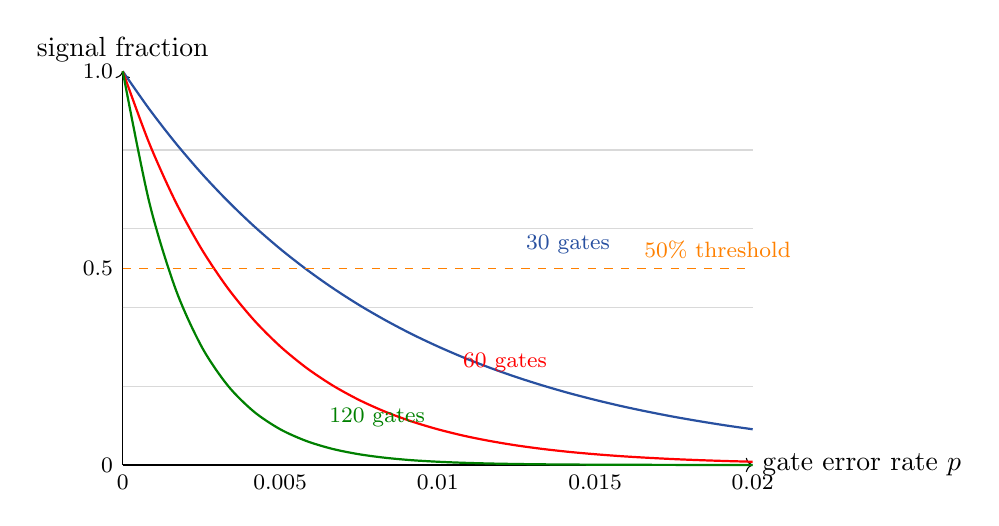
\begin{tikzpicture}
    \draw[->] (0,0) -- (8,0) node[right] {gate error rate $p$};
    \draw[->] (0,0) -- (0,5) node[above] {signal fraction};

    % Grid
    \draw[gray!30] (0,1) -- (8,1);
    \draw[gray!30] (0,2) -- (8,2);
    \draw[gray!30] (0,3) -- (8,3);
    \draw[gray!30] (0,4) -- (8,4);

    % Axis labels
    \node[below, font=\footnotesize] at (0,0) {0};
    \node[below, font=\footnotesize] at (2,0) {0.005};
    \node[below, font=\footnotesize] at (4,0) {0.01};
    \node[below, font=\footnotesize] at (6,0) {0.015};
    \node[below, font=\footnotesize] at (8,0) {0.02};
    \node[left, font=\footnotesize] at (0,0) {0};
    \node[left, font=\footnotesize] at (0,2.5) {0.5};
    \node[left, font=\footnotesize] at (0,5) {1.0};

    % Curves for different circuit sizes
    \draw[circuitblue, thick] plot[smooth, domain=0:8]
        (\x, {5*exp(-\x*0.3)});
    \node[circuitblue, right, font=\footnotesize] at (5, 2.8) {30 gates};

    \draw[red, thick] plot[smooth, domain=0:8]
        (\x, {5*exp(-\x*0.6)});
    \node[red, right, font=\footnotesize] at (4.2, 1.3) {60 gates};

    \draw[green!50!black, thick] plot[smooth, domain=0:8]
        (\x, {5*exp(-\x*1.2)});
    \node[green!50!black, right, font=\footnotesize] at (2.5, 0.6) {120 gates};

    % Threshold line
    \draw[dashed, orange] (0, 2.5) -- (8, 2.5);
    \node[orange, above right, font=\footnotesize] at (6.5, 2.5) {50\% threshold};
\end{tikzpicture}
\end{center}

%% ========================================================
\section{Benchmarking: Quantum vs Classical Kernels}
%% ========================================================

lets see how quantum kernels actually perform on standard toy datasets. spoiler: on these small datasets, classical kernels r competitive or better. but the exercise is still valuable bcs it shows the full pipeline.

\subsection{The Iris Dataset}

the iris dataset: 150 samples, 4 features, 3 classes. for quantum kernels, we typically use 2 classes (setosa vs versicolor, or versicolor vs virginica) and 2 features (for 2 qubits).

\textbf{setup}: 2 qubits, ZZFeatureMap with 2 reps, 1024 shots. train/test split 70/30. compare against RBF kernel SVM.

\textbf{expected results}:
\begin{center}
\renewcommand{\arraystretch}{1.3}
\begin{tabular}{|l|c|c|}
\hline
\textbf{Kernel} & \textbf{Train Accuracy} & \textbf{Test Accuracy} \\
\hline
Quantum (ZZFeatureMap, reps=2) & $\sim 95\%$ & $\sim 93\%$ \\
\hline
Classical (RBF, $\gamma=1.0$) & $\sim 97\%$ & $\sim 95\%$ \\
\hline
Classical (polynomial, deg=3) & $\sim 96\%$ & $\sim 93\%$ \\
\hline
Classical (linear) & $\sim 88\%$ & $\sim 87\%$ \\
\hline
\end{tabular}
\end{center}

the quantum kernel is competitive with the polynomial kernel but slightly below RBF. this is typical --- on easy datasets with few features, classical kernels have been optimized for decades and work great.

\subsection{The Moons Dataset}

make\_moons from sklearn: 200 samples, 2 features, 2 classes, with noise=0.2. this is a classic nonlinear classification problem.

\textbf{setup}: 2 qubits, ZZFeatureMap with 2 reps, 1024 shots.

\textbf{expected results}:
\begin{center}
\renewcommand{\arraystretch}{1.3}
\begin{tabular}{|l|c|c|}
\hline
\textbf{Kernel} & \textbf{Train Accuracy} & \textbf{Test Accuracy} \\
\hline
Quantum (ZZFeatureMap, reps=1) & $\sim 85\%$ & $\sim 83\%$ \\
\hline
Quantum (ZZFeatureMap, reps=2) & $\sim 92\%$ & $\sim 90\%$ \\
\hline
Quantum (ZZFeatureMap, reps=3) & $\sim 95\%$ & $\sim 91\%$ \\
\hline
Classical (RBF, tuned) & $\sim 97\%$ & $\sim 95\%$ \\
\hline
\end{tabular}
\end{center}

\begin{intuition}
on moons, the quantum kernel with enough reps gets close to RBF but doesnt beat it. the reason: the moons dataset has a simple nonlinear structure that RBF captures perfectly. the quantum kernel introduces more complex features that r partly relevant but also partly noise.
\end{intuition}

\subsection{The Circles Dataset}

make\_circles from sklearn: 200 samples, 2 features, 2 classes, with noise=0.15. concentric circles --- another classic nonlinear problem.

\textbf{expected results}:
\begin{center}
\renewcommand{\arraystretch}{1.3}
\begin{tabular}{|l|c|c|}
\hline
\textbf{Kernel} & \textbf{Train Accuracy} & \textbf{Test Accuracy} \\
\hline
Quantum (ZZFeatureMap, reps=2) & $\sim 88\%$ & $\sim 86\%$ \\
\hline
Quantum (ZFeatureMap, reps=2) & $\sim 75\%$ & $\sim 73\%$ \\
\hline
Classical (RBF) & $\sim 95\%$ & $\sim 93\%$ \\
\hline
Classical (polynomial, deg=2) & $\sim 93\%$ & $\sim 91\%$ \\
\hline
\end{tabular}
\end{center}

\begin{keypoint}
the circles dataset shows why ZFeatureMap (no entanglement) is bad --- it cant capture the radial structure. ZZFeatureMap does better bcs the entangling gates create features that can separate circles, but RBF is still better bcs its literally designed for radial problems ($k(\mathbf{x}, \mathbf{x}') = e^{-\gamma \|\mathbf{x} - \mathbf{x}'\|^2}$).
\end{keypoint}

\subsection{Interpreting Kernel Matrices}

wt does a good vs bad kernel matrix look like?

\textbf{good kernel matrix}:
\begin{itemize}[leftmargin=*]
    \item clear block structure: points in the same class have high kernel values, points in different classes have low kernel values
    \item smooth variation: nearby points (in the same class) have similar kernel values
    \item well-conditioned: eigenvalues span a reasonable range, not all clustered near zero
\end{itemize}

\textbf{bad kernel matrix}:
\begin{itemize}[leftmargin=*]
    \item no block structure: kernel values r random regardless of class labels
    \item diagonal dominance: $K_{ii} \gg K_{ij}$ for all $i \neq j$ (the kernel is too ``sharp'')
    \item all entries similar: $K_{ij} \approx c$ for all $i,j$ (the kernel doesnt discriminate, often happens with too many qubits)
    \item heavy noise: lots of random variation in entries
\end{itemize}

conceptually, a kernel matrix heatmap for binary classification should look smtg like this:

\begin{center}
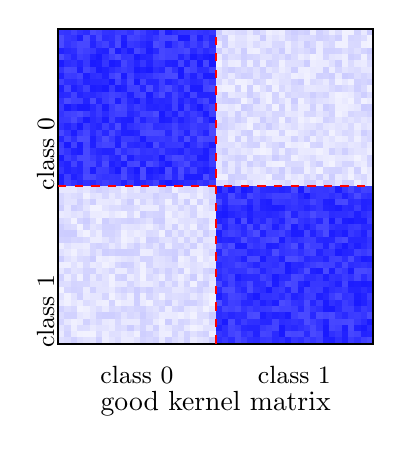
\begin{tikzpicture}[scale=0.08]
    % Good kernel - class 0 block (top-left)
    \foreach \i in {0,...,24} {
        \foreach \j in {0,...,24} {
            \pgfmathsetmacro{\val}{70 + 20*rnd}
            \fill[blue!\val!white] (\i, 49-\j) rectangle (\i+1, 50-\j);
        }
    }
    % Good kernel - class 1 block (bottom-right)
    \foreach \i in {25,...,49} {
        \foreach \j in {25,...,49} {
            \pgfmathsetmacro{\val}{70 + 20*rnd}
            \fill[blue!\val!white] (\i, 49-\j) rectangle (\i+1, 50-\j);
        }
    }
    % Off-diagonal blocks (low values)
    \foreach \i in {0,...,24} {
        \foreach \j in {25,...,49} {
            \pgfmathsetmacro{\val}{5 + 15*rnd}
            \fill[blue!\val!white] (\i, 49-\j) rectangle (\i+1, 50-\j);
        }
    }
    \foreach \i in {25,...,49} {
        \foreach \j in {0,...,24} {
            \pgfmathsetmacro{\val}{5 + 15*rnd}
            \fill[blue!\val!white] (\i, 49-\j) rectangle (\i+1, 50-\j);
        }
    }

    \draw[thick] (0,0) rectangle (50,50);
    \draw[dashed, red, thick] (25, 0) -- (25, 50);
    \draw[dashed, red, thick] (0, 25) -- (50, 25);

    \node[below, font=\small] at (12.5, -2) {class 0};
    \node[below, font=\small] at (37.5, -2) {class 1};
    \node[left, font=\small, rotate=90] at (-2, 37.5) {class 0};
    \node[left, font=\small, rotate=90] at (-2, 12.5) {class 1};
    \node[below, font=\normalsize] at (25, -6) {good kernel matrix};
\end{tikzpicture}
\end{center}

%% ========================================================
\section{Results Interpretation Guidelines}
%% ========================================================

when u run quantum kernel experiments, here is how to interpret wt u see:

\subsection{Kernel Matrix Diagnostics}

\begin{enumerate}[leftmargin=*]
    \item \textbf{check the diagonal}: should all be 1.0 (or very close). if not, smtg is wrong with ur implementation.

    \item \textbf{check the off-diagonal range}: values should span a meaningful range, say $[0.01, 0.8]$. if everything is near 0, ur kernel is too ``spread out'' (too many qubits or too much entanglement). if everything is near 1, ur kernel is too ``narrow'' (features r not being differentiated).

    \item \textbf{compute alignment}: alignment above $0.1$ is decent for a random feature map. above $0.3$ is good. above $0.5$ is excellent.

    \item \textbf{eigenvalue spectrum}: compute eigenvalues of $K$. a good kernel has a few large eigenvalues and many small ones (low effective rank). this means the kernel is capturing a few important directions in feature space. if all eigenvalues r similar, the kernel is essentially random.

    \item \textbf{compare with ideal}: compute the ideal kernel $K^* = \mathbf{y}\mathbf{y}^\top$ and visually compare. the closer ur kernel looks to this, the better.
\end{enumerate}

\subsection{When Quantum Kernels Work Well}

based on current research, quantum kernels tend to work well when:
\begin{itemize}[leftmargin=*]
    \item the data has structure that maps naturally to quantum correlations (e.g., data generated by quantum processes)
    \item the feature dimension matches the number of available qubits
    \item the dataset is small enough that $O(M^2)$ kernel evaluations r feasible
    \item the circuit depth is manageable given hardware noise
\end{itemize}

\subsection{When Quantum Kernels Struggle}

\begin{itemize}[leftmargin=*]
    \item large datasets ($M > 500$): the $O(M^2)$ cost becomes prohibitive
    \item high-dimensional data requiring many qubits: kernel concentration kills performance
    \item noisy hardware with deep circuits: noise washes out the signal
    \item problems where classical kernels (especially RBF) already work perfectly
\end{itemize}

%% ========================================================
\section{Advanced: Projected Quantum Kernels}
%% ========================================================

one way to mitigate the kernel concentration problem is to use \emph{projected quantum kernels} (huang et al., 2021).

\begin{definition}[Projected Quantum Kernel]
instead of computing the full state fidelity, project the quantum state onto local subsystems:
\[
\kappa_{\text{proj}}(\mathbf{x}, \mathbf{x}') = \exp\!\left(-\gamma \sum_{S} \left\| \rho_S(\mathbf{x}) - \rho_S(\mathbf{x}') \right\|_F^2 \right)
\]
where $\rho_S(\mathbf{x}) = \text{Tr}_{\bar{S}}[\ket{\phi(\mathbf{x})}\bra{\phi(\mathbf{x})}]$ is the reduced density matrix on subsystem $S$.
\end{definition}

the key differences from standard quantum kernels:
\begin{enumerate}[leftmargin=*]
    \item measures local properties (1 or 2 qubit reduced states) instead of global fidelity
    \item doesnt suffer from exponential concentration bcs local observables have $O(1)$ variance
    \item can be computed from local measurements: measure each qubit (or pair) in $X$, $Y$, $Z$ bases
    \item the resulting kernel is guaranteed to be PSD (its a gaussian kernel on measured features)
\end{enumerate}

the local measurement approach:
\begin{align}
\rho_i(\mathbf{x}) &\to (\langle X_i \rangle, \langle Y_i \rangle, \langle Z_i \rangle) \in \mathbb{R}^3 \\
\rho_{ij}(\mathbf{x}) &\to (\langle X_i X_j \rangle, \langle X_i Y_j \rangle, \ldots, \langle Z_i Z_j \rangle) \in \mathbb{R}^9
\end{align}

this gives a classical feature vector of dimension $3n + 9\binom{n}{2}$ that captures the essential quantum information without the concentration problem.

\begin{intuition}
projected quantum kernels r like a compromise: u use the quantum circuit to create complex features, but then u extract classical summary statistics from the quantum state. its less ``quantum'' than full fidelity kernels, but it actually works better in practice on noisy hardware.
\end{intuition}

%% ========================================================
\section{Complete Workflow Diagram}
%% ========================================================

here is the complete workflow for a quantum kernel experiment, showing all the steps from problem definition to results:

\begin{center}
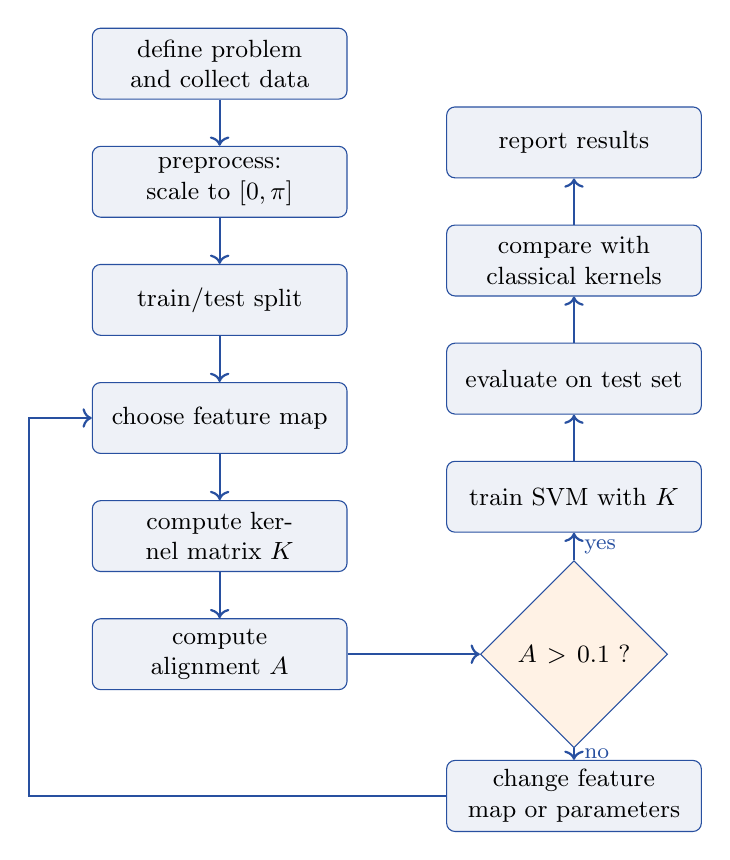
\begin{tikzpicture}[
    node distance=1.5cm and 2cm,
    block/.style={rectangle, draw=circuitblue, fill=circuitblue!8,
        minimum width=3.2cm, minimum height=0.9cm, rounded corners=3pt,
        font=\small, text width=3cm, align=center},
    decision/.style={diamond, draw=circuitblue, fill=orange!10,
        minimum width=2cm, minimum height=1cm,
        font=\small, text width=2cm, align=center, inner sep=1pt},
    arrow/.style={->, thick, circuitblue}
]
    % Column 1
    \node[block] (prob) {define problem and collect data};
    \node[block, below of=prob] (pre) {preprocess: scale to $[0,\pi]$};
    \node[block, below of=pre] (split) {train/test split};
    \node[block, below of=split] (fm) {choose feature map};
    \node[block, below of=fm] (kern) {compute kernel matrix $K$};
    \node[block, below of=kern] (align) {compute alignment $A$};

    % Column 2
    \node[decision, right of=align, xshift=3cm] (check) {$A > 0.1$ ?};
    \node[block, above of=check, yshift=0.5cm] (train) {train SVM with $K$};
    \node[block, above of=train] (eval) {evaluate on test set};
    \node[block, above of=eval] (compare) {compare with classical kernels};
    \node[block, above of=compare] (report) {report results};

    % Back arrow for bad alignment
    \node[block, below of=check, yshift=-0.3cm] (change) {change feature map or parameters};

    \draw[arrow] (prob) -- (pre);
    \draw[arrow] (pre) -- (split);
    \draw[arrow] (split) -- (fm);
    \draw[arrow] (fm) -- (kern);
    \draw[arrow] (kern) -- (align);
    \draw[arrow] (align) -- (check);
    \draw[arrow] (check) -- node[right, font=\footnotesize] {yes} (train);
    \draw[arrow] (train) -- (eval);
    \draw[arrow] (eval) -- (compare);
    \draw[arrow] (compare) -- (report);
    \draw[arrow] (check) -- node[right, font=\footnotesize] {no} (change);
    \draw[arrow] (change.west) -| ([xshift=-0.8cm]fm.west) -- (fm.west);
\end{tikzpicture}
\end{center}

%% ========================================================
\section{Benchmarking Strategy}
%% ========================================================

when benchmarking quantum kernels, u need a systematic approach. here is the recommended protocol:

\subsection{Experimental Setup}

\begin{enumerate}[leftmargin=*]
    \item \textbf{datasets}: use at least 3 datasets with different characteristics (linear, nonlinear, multi-class reduced to binary)

    \item \textbf{quantum kernels to test}:
    \begin{itemize}[leftmargin=*]
        \item ZFeatureMap (baseline, should match classical)
        \item ZZFeatureMap with reps = 1, 2, 3
        \item PauliFeatureMap with different paulis
    \end{itemize}

    \item \textbf{classical kernels to compare}:
    \begin{itemize}[leftmargin=*]
        \item linear kernel (baseline)
        \item RBF kernel with tuned $\gamma$
        \item polynomial kernel with tuned degree
    \end{itemize}

    \item \textbf{metrics}: accuracy, F1-score, kernel alignment, training time, total quantum cost (circuits $\times$ shots)

    \item \textbf{repetitions}: run each experiment 5-10 times with different random train/test splits to get error bars
\end{enumerate}

\subsection{Fair Comparison Guidelines}

\begin{keypoint}
a fair comparison requires:
\begin{itemize}[leftmargin=*]
    \item same train/test splits for quantum and classical
    \item hyperparameter tuning for both quantum (reps, entanglement) and classical ($C$, $\gamma$, degree)
    \item same evaluation metrics
    \item reporting of computational cost (quantum kernels r much slower)
\end{itemize}
dont cherry-pick the one run where quantum beats classical. report averages and standard deviations.
\end{keypoint}

%% ========================================================
\section{Common Pitfalls}
%% ========================================================

from experience (and from reading a lot of quantum kernel papers), here r the most common mistakes:

\begin{enumerate}[leftmargin=*]
    \item \textbf{forgetting to normalize}: raw features in different ranges lead to rotation gates that dont use the full bloch sphere. always preprocess.

    \item \textbf{too many qubits}: using 10+ qubits for a dataset with 2 useful features. the extra qubits just add noise and cause concentration.

    \item \textbf{too many reps}: more reps = more expressivity, but also more noise sensitivity and slower execution. start with reps=2.

    \item \textbf{not enough shots}: below 512 shots, the kernel matrix is dominated by statistical noise. use at least 1024.

    \item \textbf{not checking PSD}: the estimated kernel matrix might not be positive semi-definite. sklearn's SVM will still run but might give weird results. always check and fix.

    \item \textbf{comparing unfairly}: comparing an untuned quantum kernel against an untuned classical kernel (or worse, against a tuned one). always tune both.

    \item \textbf{ignoring the cost}: claiming quantum is ``comparable'' to classical while ignoring that the quantum kernel took 1000x more compute. always report cost.

    \item \textbf{overfitting with deep kernels}: very expressive quantum kernels can perfectly fit the training data but generalize poorly. monitor the train/test gap.
\end{enumerate}

%% ========================================================
\section{Summary and Key Takeaways}
%% ========================================================

this lecture covered the practical side of quantum kernels. lets recap:

\begin{enumerate}[leftmargin=*]
    \item \textbf{the pipeline is straightforward}: data $\to$ normalize $\to$ feature map $\to$ kernel matrix $\to$ SVM $\to$ predictions. qiskit's \texttt{FidelityQuantumKernel} handles the quantum parts.

    \item \textbf{feature map choice matters a lot}: ZFeatureMap gives u a classical kernel. ZZFeatureMap is the standard for potentially quantum advantage. entanglement is necessary but not sufficient.

    \item \textbf{kernel computation is expensive}: $O(M^2)$ circuits, each with many shots. the total cost scales quadratically with dataset size.

    \item \textbf{noise degrades kernel quality}: the signal fraction drops exponentially with circuit depth and gate error rate. shallow circuits r preferable on current hardware.

    \item \textbf{kernel alignment is ur best friend}: it tells u quickly whether a kernel is good for ur task without doing full SVM training.

    \item \textbf{on toy datasets, classical wins or ties}: this is expected. the real question is whether quantum kernels can solve problems that classical kernels genuinely cant (next lecture).

    \item \textbf{projected quantum kernels}: a practical compromise that avoids concentration and works better on noisy hardware.
\end{enumerate}

next lecture well go deeper into QSVC, QSVR, and the pegasos algorithm, plus tackle real datasets and do proper cross-validation and hyperparameter tuning.

\end{document}
